\subsection{EtherCAT}
%zasada działania
%topologia
%źródła opóźnień
%wady/zalety
%itd.
%%%%%%%%%%%%%%%%%%%%%%%%%%%%%%%%%%%%%%%%%%%%%%%%%%%%%%%%%%%%%%%%%%%%%%%%%%%%%%%%%%%%%%%%%%%

EtherCAT jest nowoczesnym protokołem sieciowym przeznaczonym do stosowania w~aplikacjach przemysłowych, szczególnie takich, które wymagają działania całego systemu w~czasie rzeczywistym. Nazwa standardu jest skrótem od hasła: „Ethernet for Control Automation Technology”. W~zakresie warstwy fizycznej bazuje na~Ethernecie. Dodatkowo zaimplementowano w!nim mechanizmy w zakresie organizacji transmisji danych pozwalające na!ominięcie głównych ograniczeń sieci Ethernet. Dzięki temu EtherCAT jest obecnie jednym z~popularniejszych oraz szybciej rozwijających się protokołów komunikacyjnych w przemyśle.

\subsubsection{Przetwarzanie ,,w locie''}
W dużej części aplikacji przemysłowych dane mają mały rozmiar rzędu pojedynczych bajtów. Wykorzystując standardowy Ethernet i~jego ramki stosunek danych użytecznych do narzutu protokołu jest bardzo nie korzystny. 
W~celu zapewnienie determinizmu oraz zwiększenia przepustowości stosuje się w~standardach przemysłowych różne rozwiązania. Jednym z przykładów jest zastępowanie procedury dostępu do medium transmisyjnego z~wykorzystaniem wielodostępu z~wykrywaniem nośnej oraz detekcją kolizji (ang. Carrier Sense Multiple Access/with Collision Detection w~skrócie CSMA/CD) na m.in mechanizm odpytywania.
Nie jest istotnym jaką metodę dokładnie zastosujemy dopóki ramki są rozsyłane pojedynczo z oraz do urządzeń. Działania te nie wyeliminuje problemu marnowania przepustowości kanału transmisyjnego i jego wykorzystania. Dlatego ten właśnie element transmisji danych z wykorzystaniem Ethernetu został potraktowany bardzo szczególnie przy projektowaniu standardu EtherCAT.

Zatem zamiast standardowej dla Ethernetu transmisji pakietowej z~koniecznością odtwarzania pofragmentowanych danych zastosowano mechanizm wykorzystujący telegramy zbudowane z datagramów, które są szczegółowe opisane w podrozdziale~\ref{subsec:telegram} .
Rozwiązanie to~polega na tym, że w pojedynczej ramce są zawarte informacje przeznaczone dla wielu różnych węzłów podrzędnych. Transmisja takiej ramka inicjowana jest przez węzeł nadrzędny, a~następnie przechodzi ona przez kolejne węzły podrzędne sieci, które przetwarzają ją w locie. W takim podejściu twórcy standardu EtherCAT potraktowali ramkę ethernetową jak pewnego rodzaju pamięć RAM, do której zapisywane i z~której odczytywane są dowolne informacje w~oparciu o~adresy lokalizujące pożądane dane w~tej pamięci.
Przetwarzanie to polega, że w~momencie odebrania ramki sprawdzane jest czy znajduje się w~niej informacja przeznaczona dla tego właśnie węzła. Jeżeli zostanie wykryte, że~tak~jest  to węzeł odczytuje odpowiedni fragment danych oraz uzupełnia ewentualnie ją o~informacje potwierdzające odbiór lub~inne wymagane przez węzeł nadrzędny. Następnie ramka jest przesyłana do kolejnego w topologi węzła lub zawraca jeśli dany węzeł jest ostatnim w~sieci. 

Dzięki takiemu podejściu protokół charakteryzuje się bardzo dużym wykorzystaniem kanału transmisyjnego w porównaniu do odpytywania w przedziale czasowym (ang. Pooling Timeslicing) oraz nadawania Master/Slave (ang. Broadcast Master/Slave) znanych ze~zwykłego EThernetu co pokazano na Rysunku~\ref{etherCAT:wykorzystanie}
\begin{figure}[htbp]
 \centering
\begin{tikzpicture}
\begin{axis}[
		ybar stacked,
		ymin=0,ymax=110, 
		yticklabels={0\%, 20\%, 40\%, 60\%, 80\%, 100\%},
		xtick=data,
		xticklabel style={text centered, text width=2.5cm},
	    xticklabels={Pooling Timeslicing, Broadcast Master/Slave, EtherCAT},
		every node near coord/.style={font=\tiny},
	    ]  
	    
\addplot[fill=gray!50] coordinates
{(1,2) (2,20) (3,0)};
\addplot[fill=yellow!50] coordinates
{(1,0) (2,0) (3,80)};
\addplot[fill=gray!80] coordinates
{(1,3) (2,10) (3,0)};
\addplot[fill=yellow!80] coordinates
{(1,0) (2,0) (3,17)};

\node[above] at ($(axis cs:1,5)$) {2-5\%};
\node[above] at ($(axis cs:2,30)$) {20-30\%};
\node[above] at ($(axis cs:3,96)$) {90-97\%};
\end{axis}

\end{tikzpicture}
\caption{Współczynnik wykorzystania kanału transmisyjnego w Ethernecie (dwa pierwsze wykresy od lewej strony) i EtherCAT}
\label{etherCAT:wykorzystanie}
\end{figure}

Wydajność tego rozwiązania jest dosyć duża, choć zależy od~liczby elementów podłączonych do sieci. W~praktyce czas opóźnienia nie wzrasta powyżej 1~ms i~zazwyczaj jest znacznie (kilku- lub kilkunastokrotnie) krótszy. Czas synchronizacji nie przekracza 1~$\mu s$. Niniejsza praca miała na celu przebadanie i~sprawdzenie czy faktycznie protokół działa tak dobrze jak zapewniają jego twórcy.

Bardzo ważnym elementem węzła sieci jest tak zwana jednostka zarządzania pamięcią FMMU (ang. fieldbus memory management unit). Odpowiada ona między innymi za uniezależnienie szybkości transferu danych od wydajności i~mocy obliczeniowej jednostki lokalnej CPU, kontrolę ruchu bez opóźnień oraz za~odwzorowanie adresu logicznego na~adres fizyczny.

\subsubsection{Telegram EtherCAT}
\label{subsec:telegram}
Jak pokazano na Rysunku~\ref{etherCAT:ramka}, telegram EtherCAT jest upakowany w  ramce Ethernet i  zawiera jeden lub więcej datagramów EtherCAT dostarczanych do urządzeń podrzędnych. Dane pomiędzy węzłami są~przekazywane jako obiekty danych procesowym (ang. process data objects, w skrócie PDO). Każdy obiekt tego typu zawiera adres konkretnego węzła lub kilku węzłów typu slave.
\begin{figure}[htbp]
 \centering
        \tikzstyle{background grid}=[draw, black!50,step=.25cm]
	\begin{tikzpicture}[node distance=2mm, auto]%, show background grid]
	\tikzset{
    	mynode/.style={rectangle,rounded corners,draw=black, top color=white, very thick, inner sep=4mm, 		text centered,font=\footnotesize},
    	mynodemini/.style={rectangle,rounded corners,draw=black, top color=white, thick, inner sep=2mm, text centered,font=\scriptsize},    	
	    myarrow/.style={->, >=latex', shorten >=1pt, ultra thick},
	    myline/.style={-, =latex', shorten >=1pt, rounded corners, ultra thick},
	    mylabel/.style={text centered, font=\scriptsize\bfseries} 
	} 
	\node[bottom color=gray!50, mynode] (ethhdr) {Ethernet header};  
	\node[bottom color=gray!50, mynodemini, below=of ethhdr.205] (da) {DA};
	\node[mylabel, below=1mm of da] (das) {6B};	
	\node[bottom color=gray!50, mynodemini, right=of da] (sa) {SA};  
	\node[mylabel, below=1mm of sa] (sas) {6B};	
	\node[bottom color=gray!50, mynodemini, right=of sa] (typ) {Typ};	
	\node[mylabel, below=1mm of typ] (typs) {2/4B};	
	\node[mylabel, below=of sas] (ethhdradr) {EtherType 0x88A4};
	
	\node[bottom color=yellow!50, mynode, right=of ethhdr, text width=2cm] (ecat) {EtherCAT};
	\node[bottom color=yellow!50, mynodemini, below=of ecat, text width=2.4cm] (ecathdr) {EtherCAT header};
	\node[mylabel, below=1mm of ecathdr] (ecathdrs) {2B};
	
	\node[bottom color=yellow!50, mynode, right=of ecat, text width=6.3cm] (ecatt) {EtherCAT telegram};
	\node[bottom color=yellow!50, mynodemini, below=of ecatt.193] (ecatd1) {Datagram 1};  	 
	\node[mylabel, below=1mm of ecatd1] (ecatd1s) {(10+n+2)B};
	\node[bottom color=yellow!50, mynodemini, right=of ecatd1] (ecatd2) {Datagram 2};
	\node[mylabel, below=1mm of ecatd2] (ecatd2s) {(10+m+2)B};  	 	 		
	\node[bottom color=yellow!50, mynodemini, right=0.9cm of ecatd2] (ecatdn) {Datagram n};
	\node[mylabel, below=1mm of ecatdn] (ecatdns) {(10+k+2)B};
	\node [fit=(ecatd1s) (ecatdns) (ecatdns)] (fit) {};  
 	%\draw [decorate, xshift=-20pt,line width=4pt] (fit.south east) -- (fit.north east);
	\draw [decorate,decoration={brace,amplitude=10pt}, line width=1pt] (fit.south east) ++(-0.3,0.3) -- ++(-6.9,0) (fit.south west);		
	\node[mylabel, below=1mm of fit] (fits) {44--1498B};
			
	\node[bottom color=gray!50, mynode, right=of ecatt] (eth) {Ethernet};
	\node[bottom color=gray!50, mynodemini, below=of eth.222] (pad) {Pad.};
	\node[mylabel, below=1mm of pad] (pads) {0--32B};
	\node[bottom color=gray!50, mynodemini, right=of pad] (fcs) {FCS}; 	 
	\node[mylabel, below=1mm of fcs] (fcss) {4B}; 		
 
	\draw[myline,black,dotted] (ecatd2) -- (ecatdn); 	
	
	\node[mylabel, below=of ethhdradr] (dal) {DA -- Destination Address};
	\node[mylabel, right=of dal] (sal) {SA -- Source Address};
	\node[mylabel, right=of sal] (padl) {Pad. -- Payload};
	\node[mylabel, right=of padl] (fcsl) {FCS -- Frame Check Sequance (CRC)};			
	
\end{tikzpicture} 
\caption{Ramka w transmisji EtherCAT i~jej podział na datagramy.}
\label{etherCAT:ramka}
\end{figure} %

Dane w systemach opartych na sieciach EtherCAT mogą być przesyłane między różnymi sieciami poprzez protokół UDP, a nie tylko w ramach jednej podsieci. Tam gdzie konieczny jest routing pakietów w oparciu o~protokół IP, ramki EtherCAT są przesyłane w~ramach pakietów protokołu UDP lub TCP (Rysunki~\ref{etherCAT:ramkaUDP}~oraz~\ref{etherCAT:ramkaTCP}). Pakiety tego typu mogą zostać uformowane i nadane z wykorzystaniem zwykłych urządzeń ethernetowych, dzięki czemu możliwe jest sterowanie aparaturą polową EtherCAT z~poziomu klasycznego komputera~PC wyposażonego w~kartę sieciową.
\begin{figure}[htbp]
 \centering
        \tikzstyle{background grid}=[draw, black!50,step=.25cm]
	\begin{tikzpicture}[node distance=2mm, auto]%, show background grid]
	\tikzset{
    	mynode/.style={rectangle,rounded corners,draw=black, top color=white, very thick, inner sep=4mm, 		text centered,font=\footnotesize},
    	mynodemini/.style={rectangle,rounded corners,draw=black, top color=white, thick, inner sep=2mm, text centered,font=\scriptsize},    	
	    myarrow/.style={->, >=latex', shorten >=1pt, ultra thick},
	    myline/.style={-, =latex', shorten >=1pt, rounded corners, ultra thick},
	    mylabel/.style={text centered, font=\scriptsize\bfseries} 
	} 
	\node[bottom color=gray!50, mynode, text width=1.6cm] (ethhdr) {Ethernet header}; 
	\node[mylabel, below=1mm of ethhdr] (ethhdrs) {14/16B};		 
	\node[mylabel, below=of ethhdrs.east] (ethhdradr) {EtherType 0x0800};
	\node[mylabel, right=5mm of ethhdradr] (udpadr) {UDP Port 0x88A4};	
	
	\node[bottom color=yellow!50, mynode, right=of ethhdr, text width=1.4cm] (ip) {IP header};
	\node[mylabel, below=1mm of ip] (ips) {20B};	
	
	\node[bottom color=yellow!50, mynode, right=of ip, text width=1.5cm] (udp) {UDP header};		
	\node[mylabel, below=1mm of udp] (udps) {8B};	
		
	\node[bottom color=yellow!50, mynode, right=of udp, text width=2cm] (ecat) {EtherCAT header};
	\node[mylabel, below=1mm of ecat] (ecats) {2B};	
		
	\node[bottom color=yellow!50, mynode, right=of ecat, text width=2cm] (ecatt) {EtherCAT telegram}; 	 	  	
	\node[mylabel, below=1mm of ecatt] (ecatts) {44--1498B};	
			
	\node[bottom color=gray!50, mynode, right=of ecatt] (eth) {Ethernet}; 		
	\node[mylabel, below=1mm of eth] (eths) {4--36B};	
		
\end{tikzpicture} 
\caption{Ramka w transmisji EtherCAT z uwzględnieniem UDP i~IP.}
\label{etherCAT:ramkaUDP}
\end{figure} %
\begin{figure}[htbp]
 \centering
        \tikzstyle{background grid}=[draw, black!50,step=.25cm]
	\begin{tikzpicture}[node distance=2mm, auto]%, show background grid]
	\tikzset{
    	mynode/.style={rectangle,rounded corners,draw=black, top color=white, very thick, inner sep=4mm, 		text centered,font=\footnotesize},
    	mynodemini/.style={rectangle,rounded corners,draw=black, top color=white, thick, inner sep=2mm, text centered,font=\scriptsize},    	
	    myarrow/.style={->, >=latex', shorten >=1pt, ultra thick},
	    myline/.style={-, =latex', shorten >=1pt, rounded corners, ultra thick},
	    mylabel/.style={text centered, font=\scriptsize\bfseries} 
	} 
	\node[bottom color=gray!50, mynode, text width=2cm] (ethhdr) {Ethernet header}; 
	\node[mylabel, below=1mm of ethhdr] (ethhdrs) {14/16B};		 
	\node[mylabel, below=of ethhdrs] (ethhdradr) {EtherType 0x0800};
	\node[mylabel, below=1mm of ethhdradr] (udpadr) {TCP Port 0x88A4};	
	
	\node[bottom color=yellow!50, mynode, right=of ethhdr, text width=1.4cm] (ip) {IP header};
	\node[mylabel, below=1mm of ip] (ips) {20B};	
	
	\node[bottom color=yellow!50, mynode, right=of ip, text width=1.5cm] (udp) {UDP header};		
	\node[mylabel, below=1mm of udp] (udps) {8B};	
		
	\node[bottom color=yellow!50, mynode, right=of udp, text width=2cm] (ecat) {EtherCAT header};
	\node[mylabel, below=1mm of ecat] (ecats) {2B};	
		
	\node[bottom color=yellow!50, mynode, right=of ecat, text width=2cm] (ecatt) {EtherCAT telegram}; 	 	  	
	\node[mylabel, below=1mm of ecatt] (ecatts) {44--1498B};	
			
	\node[bottom color=gray!50, mynode, right=of ecatt] (eth) {Ethernet}; 		
	\node[mylabel, below=1mm of eth] (eths) {4--36B};	
		
\end{tikzpicture} 
\caption{Ramka w transmisji EtherCAT z uwzględnieniem TCP i~IP.}
\label{etherCAT:ramkaTCP}
\end{figure} %

Rozwiązanie to~zapewnia elastyczną komunikację pomiędzy urządzeniami pracującymi w~standardzie Ethernet oraz EtherCAT, a~także umożliwia wymianę danych pomiędzy urządzeniami znajdującymi się w segmentach sieci podłączonych do różnych routerów. W takim przypadku prędkość wymiany danych zależy w~dużym stopniu od~prędkości działania routerów, co~należy uwzględnić przy ewentualnym projektowanie systemu pracującego w~rozdzielonej sieci.

Każdy datagram EtherCAT jest komendą, która zawiera zgodnie z Rysunkiem~\ref{etherCAT:datagram} nagłówek, dane i~licznik roboczy. Nagłówek i~dane są~używane do~wyspecyfikowania operacji, które muszą być wykonane przez węzeł podrzędny, natomiast licznik roboczy jest aktualizowany przez niego informując węzeł nadrzędny, że~odebrał on i~przetwarza komendę.
\begin{figure}[htbp]
 \centering
        \tikzstyle{background grid}=[draw, black!50,step=.25cm]
	\begin{tikzpicture}[node distance=2mm, auto]%, show background grid]
	\tikzset{
    	mynode/.style={rectangle,rounded corners,draw=black, top color=white, very thick, inner sep=4mm, 		text centered,font=\footnotesize},
    	mynodemini/.style={rectangle,rounded corners,draw=black, top color=white, thick, inner sep=2mm, text centered,font=\scriptsize},    	
	    myarrow/.style={->, >=latex', shorten >=1pt, ultra thick},
	    myline/.style={-, =latex', shorten >=1pt, rounded corners, ultra thick},
	    mylabel/.style={text centered, font=\scriptsize\bfseries} 
	} 
	\node[bottom color=yellow!50, mynode] (datagram) {Datagram};  
	\node[bottom color=yellow!50, mynode, below=1cm of datagram] (part1) {Dane};   
	\node[mylabel, below=1mm of part1] (part1s) {32--1486B};				
	\node[bottom color=yellow!50, mynode, left=of part1] (part2) {Nagłówek};   	
	\node[mylabel, below=1mm of part2] (part2s) {10B};			
	\node[bottom color=yellow!50, mynode, right=of part1] (part3) {Licznik};   				
	\node[mylabel, below=1mm of part3] (part3s) {2B};	
 
	\draw[myline,black,dotted] (datagram.south west) -- (part2.north west); 	
	\draw[myline,black,dotted] (datagram.south east) -- (part3.north east); 
\end{tikzpicture} 
\caption{Budowa datagramu}
\label{etherCAT:datagram}
\end{figure} %

Nagłówek datagramu przedstawiony na Rysunku~\ref{etherCAT:datagram_header}. Jak widać składa się on ze~sporej ilości pól wymagających dokładnego objaśnienia.
\begin{description}
\item[Cmd] Typ rozkazu EtherCAT (ang. EtherCAT Command Type)
\item[Idx] Indeks jest numerycznym identyfikatorem używanym przez węzeł nadrzędny do~wykrywania zdublowanych lub zagubionych datagramów, pole~to nie~powinno być nigdy modyfikowane przez węzły podrzędne
\item[Address] Adres urządzenia zapisany w~sposób zależny od trybu adresacji
\item[Len] Długość danych zawartych w analizowanym datagramie (rozmiar pola danych)
\item[R] Pole zarezerwowane, powinno mieć zawsze wartość 0
\item[C] Pole zabezpieczające ramkę przed zapętleniem\\
0: oznacza, że przetwarzana ramka nie jest zapętlona \\
1: oznacza, że za przetwarzana ramka wykonała już jeden obieg pętli
\item[M] Pole to określa czy w~aktualnie przetwarzanym telegramie są kolejne datagramy \\
0: oznacza, że przetwarzany datagram jest ostatni \\
1: oznacza, że za przetwarzanym datagramem są kolejne
\item[IRQ] Pole żądania zdarzeń od węzłów podrzędnych, pole jest wynikiem sumy logicznej (ang. logical OR) żądań wszystkich węzłów podrzędnych
\end{description}

\begin{figure}[htbp]
 \centering
        \tikzstyle{background grid}=[draw, black!50,step=.25cm]
	\begin{tikzpicture}[node distance=2mm, auto]%, show background grid]
	\tikzset{
    	mynode/.style={rectangle,rounded corners,draw=black, top color=white, very thick, inner sep=4mm, 		text centered,font=\footnotesize},
    	mynodemini/.style={rectangle,rounded corners,draw=black, top color=white, thick, inner sep=2mm, text centered,font=\scriptsize},    	
	    myarrow/.style={->, >=latex', shorten >=1pt, ultra thick},
	    myline/.style={-, =latex', shorten >=1pt, rounded corners, ultra thick},
	    mylabel/.style={text centered, font=\scriptsize\bfseries} 
	} 
	\node[bottom color=yellow!50, mynode] (header) {Nagłówek datagramu};  
	\node[bottom color=yellow!50, mynode, below=1cm of header.south west, text width=3.2cm] (mainadress) {Address};	
	\node[mylabel, above=1mm of mainadress] (mainadresss) {4B};		
	\node[bottom color=yellow!50, mynode, below=2cm of mainadress.25] (offset) {Offset}; 
	\node[bottom color=yellow!50, mynode, below=1mm of offset] (offset2) {Offset}; 	
	\node[mylabel, above=1mm of offset] (offsets) {2B};		  		
	\node[bottom color=yellow!50, mynode, left=of offset] (position) {Position};
	\node[bottom color=yellow!50, mynode, below=1mm of position] (adress) {Address}; 
	\node[bottom color=yellow!50, mynode, below=1mm of adress.south east, text width=3.2cm] (ladress) {Logical Address}; 			   		
	\node[mylabel, above=1mm of position] (positions) {2B};
	
	\node[bottom color=yellow!50, mynode, left=of mainadress] (idx) {Idx};   		
	\node[mylabel, below=1mm of idx] (idxs) {1B};
	\node[bottom color=yellow!50, mynode, left=of idx] (cmd) {Cmd};   		
	\node[mylabel, below=1mm of cmd] (cmds) {1B};		
	\node[bottom color=yellow!50, mynode, right=of mainadress] (len) {Len};   				
	\node[mylabel, below=1mm of len] (lens) {11b};	
	\node[bottom color=yellow!50, mynode, right=of len] (r) {R};   				
	\node[mylabel, below=1mm of r] (rs) {3b};	
	\node[bottom color=yellow!50, mynode, right=of r] (c) {C};   				
	\node[mylabel, below=1mm of c] (cs) {1b};		
	\node[bottom color=yellow!50, mynode, right=of c] (m) {M};   				
	\node[mylabel, below=1mm of m] (ms) {1b};	
	\node[bottom color=yellow!50, mynode, right=of m] (irq) {IRQ};   				
	\node[mylabel, below=1mm of irq] (irqs) {2B};	
				 
	\draw[myline,black,dotted] (datagram.south west) -- (cmd.north west); 	
	\draw[myline,black,dotted] (datagram.south east) -- (irq.north east); 
	
	\draw[myline,black,dotted] (mainadress.south west) -- (position.north west); 	
	\draw[myline,black,dotted] (mainadress.south east) -- (offset.north east); 
		
\end{tikzpicture} 
\caption{Budowa nagłówka datagramu}
\label{etherCAT:datagram_header}
\end{figure} %

Oprócz części zawierającej dane pogrupowane w datagramy telegram EtherCAT zawiera również nagłówek, którego budowę  przedstawia Rysunek~\ref{etherCAT:header}. Pierwsze pole określa długość wszystkich datagramów w~danym telegramie, która zależy od ilości węzłów oraz długości wiadomości. Drugie pole jest bitem zarezerwowanym, a~jego wartość powinna wynosić 0. Ostatnie pole określa typ protokołu EtherCAT. Typ ten definiuje typ wiadomości, co~pozwala na prawidłową interpretację danych.
Standard przewiduje 3~dopuszczalne typy:
\begin{itemize}
\item Typ 1: Protokół EtherCAT dla urządzeń -- Wymiana Datagramów (ang. EtherCAT Device Protocol, EtherCAT Datagram(s)),
\item Typ 4: EAP Wymiana danych procesowych -- wymiany cykliczne (ang. EtherCAT Automation Protocol, Process data communications),
\item Typ 5: EAP Wymiana komunikatów na żądanie (wymiany acykliczne (ang. EtherCAT Automation Protocol, Mailbox communication).
\end{itemize}
\begin{figure}[htbp]
 \centering
        \tikzstyle{background grid}=[draw, black!50,step=.25cm]
	\begin{tikzpicture}[node distance=2mm, auto]%, show background grid]
	\tikzset{
    	mynode/.style={rectangle,rounded corners,draw=black, top color=white, very thick, inner sep=4mm, 		text centered,font=\footnotesize},
    	mynodemini/.style={rectangle,rounded corners,draw=black, top color=white, thick, inner sep=2mm, text centered,font=\scriptsize},    	
	    myarrow/.style={->, >=latex', shorten >=1pt, ultra thick},
	    myline/.style={-, =latex', shorten >=1pt, rounded corners, ultra thick},
	    mylabel/.style={text centered, font=\scriptsize\bfseries} 
	} 
	\node[bottom color=yellow!50, mynode] (header) {Nagłówek};  
	\node[bottom color=yellow!50, mynode, below=1cm of header] (part1) {Zarezerwowany}; 
	\node[mylabel, below=1mm of part1] (part1s) {1b};		  		
	\node[bottom color=yellow!50, mynode, left=of part1] (part2) {Długość};   		
	\node[mylabel, below=1mm of part2] (part2s) {11b};	
	\node[bottom color=yellow!50, mynode, right=of part1] (part3) {Typ};   				
	\node[mylabel, below=1mm of part3] (part3s) {4b};	
	 
	\draw[myline,black,dotted] (datagram.south west) -- (part2.north west); 	
	\draw[myline,black,dotted] (datagram.south east) -- (part3.north east); 
\end{tikzpicture} 
\caption{Budowa nagłówka EtherCAT}
\label{etherCAT:header}
\end{figure} %

\subsubsection{Topologia}
Kolejne ramki nadawane są przez urządzenie pełniące rolę kontrolera i~przesyłane do najbliższego urządzenia podrzędnego. Urządzenie to ma przydzielony adres, który jednoznacznie identyfikuje datagram, dzięki czemu może odczytać przeznaczone dla siebie dane. Niezależnie od tego, czy urządzenie coś zapisało, czy też tylko odczytywało fragment ramki, przesyła ją dalej do kolejnego z~urządzeń zgodnie z tym co pokazano na Rysunku~\ref{etherCAT:topologia}. Duża szybkość tej metody transmisji wynika m.in. z tego, że nie ma potrzeby dekodowania całej ramki danych. Pozwala to błyskawicznie przekazywać ramki pomiędzy urządzeniami.

\begin{figure}[htbp]
 \centering
        \tikzstyle{background grid}=[draw, black!50,step=.25cm]
	\begin{tikzpicture}[node distance=1cm, auto]%, show background grid][scale=1.1]
	\tikzset{
    	mynode/.style={rectangle,rounded corners,draw=black, top color=white, bottom color=orange!50,very thick, inner sep=0.6em, minimum size=2.5em, 		text centered, text width=2.5cm},
    	mynodemini/.style={rectangle,rounded corners,draw=black, top color=white, bottom color=orange!50,very thick, inner sep=.5em, text centered},    	
	    myarrow/.style={->, >=latex', shorten >=1pt, ultra thick},
	    myline/.style={-, =latex', shorten >=1pt, rounded corners, ultra thick},
	    mylabel/.style={text width=7em, text centered} 
	} 
	\node[mynode] (master) {Węzeł nadrzędny \\ (ang. \textit{master})};  
	\node[mynode, below right=of master] (slave1) {Węzeł podrzędny 1};
	\node[mynode, right=of slave1] (slave2) {Węzeł podrzędny 2};
	\node[mynode, right=of slave2] (slaven) {Węzeł podrzędny n};  	 	 		
	
	\draw[myarrow,black] (master.350) -| (slave1.135);
	\draw[myarrow,black] (slave1.45) -- ++(0,1.5) -| (slave2.135);
	\draw[myarrow,black,dotted] (slave2.45) -- ++(0,1.5) -| (slaven.135);	
	\draw[myarrow,black] (slaven.45) |- (master.20);	
 
\end{tikzpicture} 
\caption{Przykładowa topologia sieci.}
\label{etherCAT:topologia}
\end{figure} %

Łatwo zauważyć, że opisana procedura transmisji wymaga zastosowania topologii magistrali, która w przypadku klasycznego Ethernetu jest generalnie nieopłacalna i ma wiele wad. Problem ten został rozwiązany poprzez zwielokrotnienie portów ethernetowych instalowanych w dużej części urządzeń zgodnych z EtherCAT.
Dosyć powszechnie spotykane są urządzenia z~dwoma lub trzema portami, a~te wystarczają już do realizacji topologii gwiazdy, czy nawet zmieszanie topologii gwiazdy i~magistrali w~ramach jednej sieci i~utworzenie struktury mocno redundantnej.

\subsubsection{Warstwa fizyczna}
Jako medium komunikacyjne w~sieciach EtherCAT można wykorzystać kable miedziane (100Base-TX), światłowody (100Base-FX) lub łącze E-bus w~technologii LVDS. Te~ostatnie wprowadzono ze~względu na~to, że~transmisja w~sieciach EtherCAT często jest realizowana na~krótkich dystansach - E-bus sprawdza się w~realizacji łączności na~odległość do~około 10 m. Kable miedziane sprawdzają~się na~większych odległościach nieprzekraczających 100 metrów, natomiast użyteczna długość światłowodów może dochodzić aż do 20 kilometrów. Jedynym warunkiem związanym z~wykorzystaniem światłowodów jest obsługa pełnego dupleksu. Wymóg ten jest podyktowany faktem, że~transmisja danych jest tak szybka iż z~reguły ramka odpowiedzi dociera do urządzenia nadrzędnego zanim całe zapytanie zostanie wysłane. Z~tego powodu, aby przesył danych pomiędzy urządzenami nie był zakłócony musi istnieć możliwość jednoczesnego przekazywania informacji w dwóch kierunkach bez spadku transferu.

W~obrębie jednej sieci EtherCAT można dowolnie zmieniać medium transmisyjne zależnie od~potrzeb. Na przykład wewnatrz szafy sterowniczej gdzie występują niewielkie odległości miedzy węzłami można zastosować z powodzeniem łącze E-bus, natomiast do połączenia szafy z modułami znajdujacymi się przy maszynach wykonawczych możemy zastosować kabel miedzieny lub światłowód w~przypadku zdecydowanie większych odległości oraz prowadzenia przewodów w~otoczeniu występowania zaburzeń elektromagnetycznych. Niestety operacja takiego łączenia wymaga zastosowania dotatkowych modułów. Na przykład, aby połaczyć ze sobą swykłą skrętke miedzianą oraz przewód światłowodowy należy zastosować moduł sprzęgający EK1501 oraz terminal przyłączy EK1521 (oba produkcji firmy Beckhoff).

\subsubsection{Synchronizacja}
\showclock{4}{50}
\ClockFrametrue\ClockStyle=1\clock{12}{0}
Idealna synchronizacja elementów składowych systemu jest bardzo istotna, a szczególnie w przypadku równoległej realizacji zależnych od siebie zadań.Specjalnie opracowana dla protokołu EtherCAT technika zegara rozproszonego pozwala zsynchronizować ze sobą urządzenia z dewiacją mniejszą niż 1~$\mu s$.
\begin{figure}[htbp]
 \centering
        \tikzstyle{background grid}=[draw, black!50,step=.25cm]
	\begin{tikzpicture}[node distance=0.8cm, auto]%, show background grid]
	\tikzset{
    	mynode/.style={rectangle,rounded corners,draw=black, top color=white, bottom color=orange!50,very thick, inner sep=1em, minimum size=2.5em, 		text centered, text width=2.5cm},
    	mynodemini/.style={rectangle,rounded corners,draw=black, top color=white, bottom color=orange!50,very thick, inner sep=.5em, text centered},    	
	    myarrow/.style={-, =latex', shorten >=1pt, ultra thick, yellow},
	    myline/.style={-, =latex', shorten >=1pt, rounded corners, thick},
	    mylabel/.style={text width=7em, text centered} 
	} 
	
	\node[mynode] (master) {Węzeł nadrzędny};  
	\node[above=2mm of master](mclock){\ClockFrametrue\ClockStyle=1\clock{3}{10}};
	\node[mylabel, above=-2mm of mclock]{M};
	\draw[myline,black] (master.north) -- ++(0,0.38) (mclock.south);
	
	\node[mynode, right=of master] (slave1) {Węzeł podrzędny 1};
	\node[above=2mm of slave1](sclock1){\showclock{3}{10}};
	\node[mylabel, above=-2mm of sclock1]{S};
	\draw[myline,black] (slave1.north) -- ++(0,0.38) (sclock1.south);	

	\node[mynodemini, below=1.5cm of slave1] (io1) {I/O};
	\node[above=2mm of io1](sio1){\showclock{3}{10}};
	\node[mylabel, above=-2mm of sio1]{S};
	\draw[myline,black] (io1.north) -- ++(0,0.38) (sio1.south);	
	\node[mynodemini, right=0mm of io1] (io2) {I/O};
	\node[above=2mm of io2](sio2){\showclock{3}{10}};
	\node[mylabel, above=-2mm of sio2]{S};
	\draw[myline,black] (io2.north) -- ++(0,0.38) (sio2.south);	
	\node[mynodemini, right=0mm of io2] (io3) {I/O};
	\node[above=2mm of io3](sio3){\showclock{3}{10}};
	\node[mylabel, above=-2mm of sio3]{S};
	\draw[myline,black] (io3.north) -- ++(0,0.38) (sio3.south);	
	\node[mynodemini, right=0mm of io3] (io4) {I/O};
	\node[above=2mm of io4](sio4){\showclock{3}{10}};
	\node[mylabel, above=-2mm of sio4]{S};
	\draw[myline,black] (io4.north) -- ++(0,0.38) (sio4.south);	
						
	\node[mynode, right=of slave1] (slave2) {Węzeł podrzędny 2};
	\node[above=2mm of slave2](sclock2){\showclock{3}{10}};
	\node[mylabel, above=-2mm of sclock2]{S};
	\draw[myline,black] (slave2.north) -- ++(0,0.38) (sclock2.south);	
		
	\node[mynode, right=of slave2] (slaven) {Węzeł podrzędny n};  	 	 		
	\node[above=2mm of slaven](sclockn){\showclock{3}{10}};
	\node[mylabel, above=-2mm of sclockn]{S};
	\draw[myline,black] (slaven.north) -- ++(0,0.38) (sclock1.south);	
		
	\draw [decorate,decoration={brace, amplitude=10pt}, line width=1pt] (mclock.south) -- (sclock1.south) node[mylabel, midway, above=3mm] (deltal) {$\Delta t_1$};		
	\draw [decorate,decoration={brace, amplitude=10pt, aspect=0.7}, line width=1pt] (mclock.south) ++(0,-0.2) -- ++(8.3,0) (sclock2.south);		
	\node[mylabel, above=4.5cm of io2.east] (deltal2) {$\Delta t_2$};		
	
	\draw[myarrow] (master.east) -| (slave1.west);
	\draw[myarrow] (slave1.east)  -| (slave2.west);
	\draw[myarrow, dotted] (slave2.east) -| (slaven.west);	
	\draw[myarrow] (slave1.west) ++(0,-0.5) -| ++(-0.3,-2.36) -| (io1.west);	
 
\end{tikzpicture} 
\caption{Schemat pracy zegarów rozproszonych.}
\label{etherCAT:synchronizacja}
\end{figure} %

\subsubsection{Realizacja węzłów EtherCAT}
Wiele najprostszych i najtańszych urządzeń z interfejsem EtherCAT można zrealizować z wykorzystaniem pojedynczego układu scalonego FPGA lub ASIC. Przykładami takich prostych urządzeń z zastosowaniem tego rozwiązania są moduły wejść/wyjść cyfrowych. Tego typu węzły nie wymagają tworzenia dodatkowego oprogramowania, ponieważ cała funkcjonalność jest realizowana w~pełni sprzętowo. Uogólniona i uproszczona architektura tej metody realizacji została przedstawiona na Rysunku~\ref{etherCAT:FPGA_ASIC}.
\begin{figure}[htbp]
 \centering
        \tikzstyle{background grid}=[draw, black!50,step=.25cm]
	\begin{tikzpicture}[node distance=1cm, auto]%, show background grid]
	\tikzset{
    	mynode/.style={rectangle,rounded corners,draw=black, fill=red!15,very thick, inner sep=1.2em, minimum size=2.5em, 		text centered, text width=2.5cm},
    	mynodemini/.style={rectangle,rounded corners,draw=black, fill=red!15,very thick, inner sep=.5em, text centered, text width=2.5cm},    	
	    myarrow/.style={<->, >=latex', shorten >=1pt, ultra thick},
	    myline/.style={-, =latex', shorten >=1pt, rounded corners, ultra thick},
	    mylabel/.style={text width=7em, text centered} 
	} 
	\node[mynode] (asic_fpga) {ASIC/FPGA \\ EtherCAT};  
	\node[mylabel, left=of asic_fpga] (io) {Cyfrowe \\ wejścia/wyjścia};
	\node[mynodemini, right=of asic_fpga.north east] (layer1) {Warstwa \\ fizyczna};
	\node[right=of layer1] (empty1) {};
	\node[mynodemini, right=of asic_fpga.south east] (layer2) {Warstwa \\ fizyczna};  	 	 		
	\node[right=of layer2] (empty2) {};	

%	\draw[myarrow] (io) -- (asic_fpga);	
    \foreach \i in {-2,...,2}{% 
      \draw[myarrow] ([yshift=\i * 0.4 cm]io.east) -- ([yshift=\i * 0.4 cm]asic_fpga.west) ;}
	
	\draw[myarrow] (asic_fpga.north east) -- (layer1);	
	\draw[myarrow] (asic_fpga.south east) -- (layer2);	
				
	\draw[myarrow] (layer1) -- (empty1);	
	\draw[myarrow] (layer2) -- (empty2);	
 
\end{tikzpicture} 
\caption{Budowa węzła EtherCAT z~wykorzystaniem pojedynczego układu FPGA lub ASIC.}
\label{etherCAT:FPGA_ASIC}
\end{figure} %

Jeżeli węzeł potrzebuje dodatkowej mocy obliczeniowej lub wymaga realizacji jakiegoś złożonego oprogramowania, którego nie~da~się zrealizować w~prosty sposób sprzętowo (w układzie FPGA) do~układu ASIC/FPGA EtherCAT dołączany jest zewnętrzny procesor często wyposażony w~pamięć typu Flash tak jak na~Rysunku~\ref{etherCAT:FPGA_ASIC+proc}. Procesor taki ma zapewnić obsługę przetwarzania na~poziomie aplikacji. Niestety koszt tego typu architektury jest wyższy niż w prostszym przypadku pozbawionym zewnętrznej jednostki, ale konstruktor bazujący na tym rozwiązaniu ma większe pole manewru w~doborze procesora odpowiedniego dla wymagań i~budżetu realizowanego projektu.
\begin{figure}[htbp]
 \centering
        \tikzstyle{background grid}=[draw, black!50,step=.25cm]
	\begin{tikzpicture}[node distance=1cm, auto]%, show background grid]
	\tikzset{
    	mynode/.style={rectangle,rounded corners,draw=black, fill=red!15,very thick, inner sep=1.2em, minimum size=2.5em, 		text centered, text width=2.5cm},
    	mynodemini/.style={rectangle,rounded corners,draw=black, fill=red!15,very thick, inner sep=.5em, text centered, text width=2.5cm},    	
	    myarrow/.style={<->, >=latex', shorten >=1pt, ultra thick},
	    myline/.style={-, =latex', shorten >=1pt, rounded corners, ultra thick},
	    mylabel/.style={text width=7em, text centered} 
	} 
	\node[mynode] (asic_fpga) {ASIC/FPGA \\ EtherCAT};  
	\node[mynode, fill=blue!15, left=3cm of asic_fpga] (proc) {Procesor};
	\node[mynodemini, right=of asic_fpga.north east] (layer1) {Warstwa \\ fizyczna};
	\node[right=of layer1] (empty1) {};
	\node[mynodemini, right=of asic_fpga.south east] (layer2) {Warstwa \\ fizyczna};  	 	 		
	\node[right=of layer2] (empty2) {};	

	\draw[myarrow] (proc) -- (asic_fpga) node [midway,above] {Interfejs};		
	\draw[myarrow] (proc) -- (asic_fpga) node [midway,below=0.6cm] {hosta};		
	
	\draw[myarrow] (asic_fpga.north east) -- (layer1);	
	\draw[myarrow] (asic_fpga.south east) -- (layer2);	
				
	\draw[myarrow] (layer1) -- (empty1);	
	\draw[myarrow] (layer2) -- (empty2);	
 
\end{tikzpicture} 
\caption{Budowa węzła z~wykorzystaniem układu ASIC/FPGA EtherCAT z~dołączonym zewnętrznym procesorem.}
\label{etherCAT:FPGA_ASIC+proc}
\end{figure} %

Kolejnym możliwym do~wykorzystania rozwiązaniem jest zastosowanie układu FPGA z~wbudowanym procesorem jak na~Rysunku~\ref{etherCAT:FPGA}. Wspólną cechą przedstawionych dotychczas możliwych konstrukcji jest fakt, że~wymagają z~reguły zastosowania dwóch układów. Wynika z tego niestety, ze zajmują więcej miejsca oraz zwiększają koszty urządzenia docelowego. Alternatywą pozwalającą wyeliminować oba opisane problemy jest zastosowanie elementów jednoukładowych. Ich wykorzystanie pozwala zredukować całkowity koszt konstrukcji nawet o 30\%.
\begin{figure}[htbp]
 \centering
        \tikzstyle{background grid}=[draw, black!50,step=.25cm]
        % Define a few styles and constants
	\tikzstyle{red}=[draw, fill=red!30, text width=5em, text centered, very thick]
	\tikzstyle{naveqs} = [red, text width=6em, fill=white!20, minimum height=1.8cm, rounded corners, very thick]
	\tikzset{
    	mynode/.style={rectangle,rounded corners,draw=black, fill=red!15,very thick, inner sep=1em, minimum size=2.5em, 		text centered, text width=2.5cm},
    	mynodemini/.style={rectangle,rounded corners,draw=black, fill=red!15,very thick, inner sep=.5em, text centered, text width=2.5cm},    	
	    myarrow/.style={<->, >=latex', shorten >=1pt, ultra thick},
	    myline/.style={-, =latex', shorten >=1pt, rounded corners, ultra thick},
	    mylabel/.style={text width=7em, text centered} 
	} 
	    
    \def\blockdist{1.6}
	\def\edgedist{2.5}

\begin{tikzpicture}
    \node (core) [naveqs] {Rdzeń ARM Cortex-A8};
    \node (memory) [naveqs, below=1mm of core] {Pamięć};    
    % Note the use of \path instead of \node at ... below. 
    \path (core.north east)+(\blockdist,-0.45) node (mi) [red] {MIII x2};
    \path (core.east)+(\blockdist,-0.3) node (uart) [red] {UART};
    \path (core.south east)+(\blockdist,-0.2) node (pru) [red] {PRU x2};

    \node (IMU) [below of=pru, text centered, text width=2cm] {Jednostka \\ PRU};
    \path (core.north)+(1.5, 0.45) node (INS) {AM335x};
    
	\node[mynodemini, right=6cm of core.east] (layer1) {Warstwa \\ fizyczna};
	\node[right=of layer1] (empty1) {};
	\node[mynodemini, right=6cm of memory.east] (layer2) {Warstwa \\ fizyczna};  	 	 		
	\node[right=of layer2] (empty2) {};	
	
	\draw[myarrow] (core.east) ++(3.55,0) -- (layer1);	
	\draw[myarrow] (memory.east) ++(3.55,0) -- (layer2);	
				
	\draw[myarrow] (layer1) -- (empty1);	
	\draw[myarrow] (layer2) -- (empty2);  
	  
    % Now it's time to draw the colored IMU and INS rectangles.
    % To draw them behind the blocks we use pgf layers. This way we  
    % can use the above block coordinates to place the backgrounds   
    \begin{pgfonlayer}{background}
        % Compute a few helper coordinates
        \path (core.north |- mi.east)+(5,1.2) node (a) {};        
        \path (INS.south -| memory.west)+(-0.5,-4.2) node (b) {};
        \path[fill=blue!15,rounded corners, draw=black!100, very thick]
            (a) rectangle (b);
            
        \path (mi.north west)+(-0.2,0.2) node (a) {};
        \path (IMU.south -| mi.east)+(+0.2,-0.2) node (b) {};
        \path[fill=red!15,rounded corners, draw=black!100, very thick]
            (a) rectangle (b);
    \end{pgfonlayer}
\end{tikzpicture}

\caption{Budowa układu FPGA z wbudowanym procesorem.}
\label{etherCAT:FPGA}
\end{figure} %

Jednym z~przykładów opisanego jednoukładowego rozwiązania~są mikrokontrolery z~rdzeniem ARM~Cortex-A8 z~rodziny Sitara AM335x produkowanymi przez amerykańską firmę Texas Instruments (Rysunek~\ref{etherCAT:Sitara}). Kluczowym elementem takiego scalaka jest programowalna jednostka czasu rzeczywistego (ang. programmable real-time unit, w~skrócie PRU). 

W~PRU zaimplementowana została warstwa MAC standardu EtherCAT. Dzięki temu odpowiada~ona bezpośrednio za~przetwarzanie przepływających przez nią telegramów, dekodowanie adresów urządzeń oraz wykonywanie zapisanych w datagramie komend. W~wyniku takiego rozwiązania, że~wszystkie założenia oraz cała funkcjonalność jest realizowana właśnie przy użyciu opisywanego PRU, zamontowany wewnątrz procesor może~być zastosowany do~realizacji bardziej zaawansowanych oraz złożonych zadań wynikających ze~specyfiki konkretnego sprzętu.
\begin{figure}[htbp]
 \centering
        \tikzstyle{background grid}=[draw, black!50,step=.25cm]
	\begin{tikzpicture}[node distance=1cm, auto]%, show background grid]
	\tikzset{
    	mynode/.style={rectangle,rounded corners,draw=black, fill=red!15 ,very thick, inner sep=1em, minimum size=2.5em, 		text centered, text width=2.5cm},
    	mynodemini/.style={rectangle,rounded corners,draw=black, fill=red!15,very thick, inner sep=.5em, text centered, text width=2.5cm},    	
	    myarrow/.style={<->, >=latex', shorten >=1pt, ultra thick},
	    myline/.style={-, =latex', shorten >=1pt, rounded corners, ultra thick},
	    mylabel/.style={text width=7em, text centered} 
	} 
	
	\node[mynode, fill=blue!15, fit={(asic_fpga) (proc.east)}] (mikro) {}; 
	
	\node[mynode] (asic_fpga) {Interfejs \\ EtherCAT};  
	\node[mylabel, left=1mm of asic_fpga] (proc) {Procesor};	
	
	\node[mynodemini, right=2cm of asic_fpga.north east] (layer1) {Warstwa \\ fizyczna};
	\node[right=of layer1] (empty1) {};
	\node[mynodemini, right=2cm of asic_fpga.south east] (layer2) {Warstwa \\ fizyczna};  	 	 		
	\node[right=of layer2] (empty2) {};	
	
	\draw[myarrow] (asic_fpga.north east) ++(0.5,0) -- (layer1);	
	\draw[myarrow] (asic_fpga.south east) ++(0.5,0) -- (layer2);	
				
	\draw[myarrow] (layer1) -- (empty1);	
	\draw[myarrow] (layer2) -- (empty2);	
 
\end{tikzpicture} 
\caption{Budowa mikrokontrolerów Sitara AM335x firmy Texas Instruments wyposażonych w programowalną jednostkę czasu rzeczywistego (ang. programmable real-time unit, PRU), w której zaimplementowano warstwę MAC protokołu EtherCAT.}
\label{etherCAT:Sitara}
\end{figure} %

\subsubsection{EtherCAT Technology Group}
\begin{figure}[!htb] 	\centering 	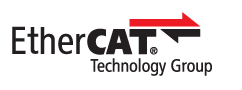
\includegraphics[width=0.3\textwidth]{images/logoETG} \caption{Logo EtherCAT Technology Group (http://www.ethercat.org).} \label{logoETG} \end{figure}

Standard EtherCAT został opracowany w~2003 roku przez Beckhoff Automation, niemiecką firmę z~branży automatyki przemysłowej. Następnie powołano organizację EtherCAT Technology Group (ETG), która zajęła~się standaryzacją tego protokołu. Stowarzyszenie~to obecnie zajmuje~się też organizowaniem szkoleń oraz popularyzacją tego standardu. 

Aktualnie w~skład ETG wchodzi ponad 2480 firm (dane na dzień 1~września~2013). Najważniejszym członkiem organizacji jest oczywiście firma BECKHOFF Automation. Pozostałe duże i~znane firmy wchodzące w~jej skład~to między innymi: ABB, Brother Industries, BMW Group, Częstochowa University of Technology, Epson, FANUC, Festo, GE Intelligent Platforms, Hitachi, Hochschule Ingolstadt, Mitsubishi, Microchip Technology, Mentor Graphics, Nikon, National Instruments, OLYMPUS, Panasonic, Rzeszów University of Technology, Red Bull Technology, Samsung Electronics, TRW Automotive, Volvo Group, Volkswagen oraz Xilinx.

Jak widać na powyższej liście w~skład organizacji wchodzą firmy z~bardzo wielu branż, a~nawet ośrodki naukowe. Autor pracy wybrał duże i~dobrze znane sobie firmy, aby pokazać jak wiele firm interesuje~się rozwojem przemysłowych protokołów komunikacyjnych.

